%!TEX root = ../plos_template.tex

\section{Genotype-phenotype maps}
The genotype of an organism has a relatively straightforward definition in terms of the sequence of nucleotides comprising its genome. Phenotypes, on the other hand, can be described at different levels of organization~\cite{Dawkins1982,Stadler2001}. The concept of phenotype was initially defined at the level of macroscopically observable physical characteristics such as shape, size, color, and various combinations thereof~\cite{Johannsen1911}. However, since the advent of molecular biology, the lowest level description of phenotype might be considered to be the dynamic phenomenon that can be described by measuring the transcription states of all genes comprising an organism's genome.  These expression levels of subsets of interacting genes determine which enzymes are produced, thus determining the rate at which metabolic reactions proceed.  These reaction rates constitute the next level of phenotypes.  These in turn determine the higher level phenotypes, ultimately culminating in macroscopic phenotypes.  In order to discuss this notion of levels of phenotypes in a mathematically precise fashion, we will develop a formal probabilistic description of the genotype-phenotype mapping that takes into account higher-order correlations among genes as well as evidence that gene expression is stochastic.

\ref{fig:expression_concept}A shows a simplified representation of a bacterial chromosome or plasmid encoding a small gene regulatory network (GRN) whose correlations strengths are not known but are to be derived from observation of the transcription process. The amount of a given transcript present in a cell given in terms of the discrete counts obtained via sequence census methods (e.g. RNA-seq) or relative abundance derived from microarray data can be binned into a smaller number of discrete classes by setting a collection of thresholds on the original data set. If only a single threshold is given, then the data can be binned into two classes depending upon whether or not the original measurement surpasses the given threshold \ref{fig:expression_concept}B.
The time series that results from such observations can be used to infer various statistics that characterize gene expression such as correlations between pairs of genes. The statistics associated to any higher-level phenotype that is determined by a particular gene expression pattern should be functions of such statistics.

If a large enough number of thresholds is available to distinguish among all possible molecule counts, then this observational protocol becomes complementary to mechanistic models.  Because there may be several sources for stochasticity in genotype-phenotype mapping including small numbers of the causal molecules and products of gene expression as well as environmental fluctuations upon which genotype-phenotype mappings are conditioned \cite{Swain2002,Paulsson2004,Thattai2004,Acar2008a,Lestas2010,Munsky2012,Chalancon2012,Neuert2013,Sanchez2013}and, regardless of the fundamental nature of stochasticity to gene expression, empirically, we observe statistical as opposed to deterministic data, we will take our model to be stochastic.  Mathematically, such a model takes the form of a Markov chain whose dynamics are governed by a master equation for the probability distributions over molecule counts.   For example, in the case of a three gene network, the master equation takes the form
$$
\frac{dP(n_1,n_2,n_3)}{dt} = \sum_{n'_1,n'_2,n'_3} M^{n_1\,n_2\,n_3}_{n'_1\,n'_2\,n'_3}(k) P(n'_1,n'_2,n'_3)
$$
where $P(n_1,n_2,n_3)$ gives the probability of observing $n_1$, $n_2$, and $n_3$ molecules of each of the three genes respectively and $M(k)$ is a Markov transition rate matrix that depends upon some rate functions $k$ that are determined by the network architecture and the dynamics of the interactions.  The solution to this equation will converge towards  a stationary distribution $P_s$ in the limit of long times. We can then coarse-grain over the molecule counts using a function that maps the states represented by vectors of integers into some other variables. For example, if $n_i$ are positive integers, then a function $f \colon \mathbb{Z}^+ \rightarrow \{0,1\}$ that takes any integer less than or equal to some threshold $T \in \mathbb{Z}^+$ to $0$ and any integer greater than $T$ to $1$ is a very simple example of such a coarse-graining. For this specific form of the coarse-graining function $f$, the coarse-grained stationary probability distribution takes the form
$$
P_s(b_1,b_2,b_3) = \sum_{n_1 \in f^{-1}(b_1)}\sum_{n_2 \in f^{-1}(b_2)}\sum_{n_3 \in f^{-1}(b_3)} P_s(n_1,n_2,n_3).
$$

At the lowest-level of the genotype-phenotype mapping, these coarse-grained expression values can be viewed as collectively determining the lowest level in the aforementioned hierarchy of phenotypes. In this way, the data derived from a number of samples of a given network can be described using binary sequences \ref{fig:expression_concept}C.  Summarizing this, we will assume that we have a set $L$ of genes and a set $P$ of coarse-grained expression levels.  Then a possible expression state of our genome is represented by a function $e : L \to P$ and coarse-graining a stationary distribution will lead to a probability distribution on the set $P^L$ of expression states.

In addition to the expression state of the whole genome, we usually will be interested in the expression states of portions of the genome.  Let $\mathcal{U}$ denote the collection of subsets of $L$ whose expression states we shall examine.  We may choose $\mathcal{U} = \mathcal{P}(L)$, the set of all subsets of $L$, or we may have $\mathcal{U}$ be a proper subset of $\mathcal{P}(L)$ because we are restricting our attention to subsets that we consider biologically relevant based upon our knowledge of a particular network (such as the relative positioning of genetic material in physical space or the manner in which genes influence each other).  For these reasons, we will require that $\mathcal{U}$ forms a topology on $L$.

Because we eventually want to compute probabilities of various sets of gene expression states, we shall introduce a sheaf of measurable spaces over $\mathcal{U}$.  The topology $\mathcal{U}$ is partially ordered under inclusion, and hence can be viewed as a category~\cite{Lane1998,MacLane1992,Awodey2006} in which the objects are open subsets of genes and morphisms represent inclusion of a smaller subset into a larger superset (i.e. $U \subseteq U' \Rightarrow U \rightarrow U'$).  Let $\mathit{Meas}$ denote the category of measurable spaces.  Recall that an object of $Meas$ is a pair $(S,\mathcal{B}(S))$ consisting of a set together with a $\sigma$-algebra over that set.  (More precisely, we will work exclusively with a subcategory of $Meas$ where the morphisms are corresponding pairs of projections on the sets and inclusions on the $\sigma$-algebras $(f:S \rightarrow S', f^{-1} : \mathcal{B}(S') \rightarrow \mathcal{B}(S))$).  Our sheaf is described by a functor $\mathcal{E} \colon \mathcal{U} \rightarrow Meas.$ which acts on objects $U$ and morphisms $U \subseteq U'$ respectively as
\begin{equation}\label{eq:gpfunctor}
\begin{split}
\mathcal{E} \colon \mathcal{U} &\rightarrow Meas,\\
U &\mapsto (P^U, \mathcal{B}(P^U)),\\
U \subseteq U' &\mapsto res^{U'}_{U}.
\end{split}
\end{equation}
So the functor $\mathcal{E}$ takes a subset of genes and returns a measurable space over the set of genotype-phenotype mappings from the given subset of genes to the set of expression levels. The restriction map operates on measurable spaces deriving from the application of $\mathcal{E}$ to a subset of genes as follows
\begin{eqnarray*}
res^{U'}_{U} \colon \mathcal{E}(U') &\rightarrow& \mathcal{E}(U)\\
(P^{U'},\mathcal{B}(P^{U'})) &\rightarrow& (P^U,\mathcal{B}(P^U))\\
(e' \colon U' \rightarrow P, S) &\mapsto& (e'|_U \colon U \rightarrow P, \bigcup_{e \in S}(e' \mapsto e'|_U)^{-1}(e))
\end{eqnarray*}

For example, if we consider the case in which we have two genes $L=\{l_1,l_2\}$ and there are two potential phenotypes, $P=\{0,1\}$, then $\mathcal{E}$ operates on the lattice of subsets generated by $L$ to give measurable spaces over the possible genotype-phenotype maps as exemplified in \ref{fig:efunctor}.

Next, we introduce probabilty distributions on this sheaf.  Recall that, if $(S,\mathcal{B}(S))$ is a measurable space, then a probability measure over $(S,\mathcal{B}(S))$ is a mapping $p \colon \mathcal{B}(S) \to [0,1]$ such that $p(S) = 1$ and $p(\bigcup_{k=1}^\infty (X_k) = \sum_{k=0}^\infty p(X_k)$ for any collection $X_k$ of pairwise disjoint elements of $\mathcal{B}(S)$.  Let $\dist((S,\mathcal{B}(S)))$ denote the set of all probability distributions over $(S,\mathcal{B}(S))$.

Furthermore, if $(S, \mathcal{B}(S))$ and $(S',\mathcal{B}(S'))$ are measurable spaces and $f:S \rightarrow S'$ is a surjection, then $f^{-1} : \mathcal{B}(S') \rightarrow \mathcal{B}(S)$ is an inclusion of measurable spaces. Given a probability distribution $p \colon \mathcal{B}(S) \to [0,1]$, the composition $p \circ f^{-1}$ is a probability distribution on $\mathcal{B}(S')$.  Let us denote this operation, which corresponds to marginalization of probabilities, as $\dist(f^{-1}) : \dist((S',\mathcal{B}(S'))) \to \dist((S,\mathcal{B}(S)))$.  With this definition, $\dist$ is a functor from the category of measurable spaces introduced in the previous section to the category $Prob$ whose objects are probability distributions and whose morphisms correspond to marginalization.

The composite $\dist \circ \expression$ is a contravariant functor from $(\mathcal{U}, \subseteq)$ to probability distributions.  However, as we shall see, this functor, unlike $\expression$, \emph{does not} satisfy the sheaf conditions and hence we only have a \emph{pre}-sheaf of probability distributions over $L$.

Finally, we introduce higher order phenotypes.  For each set of genes $U \in \mathcal{U}$, let $\phi_i (U)$ be the set of phenotypes of level $i$ whose values can be determined from the expression levels of genes in $U$.  (Note that $\phi_i (U)$ may be empty if the set $U$ does not contain enough genes to determine the values of any phenotype of level $i$.)  When $U_1 \subseteq U_2 \in \mathcal{U}$, we have a restriction map $\pi_i^{U_2 U_1} \colon \phi_i(U_2) \to \phi_1(U_2)$.  These maps satisfy the consistency conditions that $\pi_i^{UU}$ is the identity map and that $\pi_i^{U_3 U_2} \circ \pi_i^{U_2 U_1} = \pi_i^{U_3 U_1}$, i.e. $\pi_i$ is a functor on $(\mathcal{U}, \subseteq)$.  As stated earlier, we set $\phi_1 (U) = P^U$ and $\pi_1^{U_2 U_1}$ to be the restriction map from $P^{U_2}$ to $P^{U_1}$.  If $i \le j$, let $\Omega_{ij}(U) : \phi_i(U) \to \phi_j(U)$ be the coarse-graining map which describes how higher level phenotypes are determined from lower level phenotypes.  These maps are all surjctions and, for consistency, we will require the following conditions:
\begin{enumerate}
\item $\Omega_{ij}(U) \circ \Omega_{jk}(U) = \Omega_{ik}(U)$ whenever $i \le j \le k$.
\item $\Omega_{ii}(U)$ is the identity map on $\phi_i (U)$.
\item If $U_1 \subseteq U_2 \in \mathcal{U}$ and $i > j$, then $\Omega_{ij}(U_1) \circ \pi_i^{U_2 U_1} = \pi_j^{U_2 U_1} \circ \Omega_{ij}(U_2)$
\end{enumerate}
In other words, $\Omega$ must be suitably functorial in both of its arguments.

Since the map $\Omega_{1i}(U)$ is a surjection from $P^U$ onto $\phi_i(U)$, we can use it to map our probabilistic structures to $\phi_i(U)$.  Set $\mathcal(E)_i = \Omega_{1i}(U)^{-1} \circ \mathcal(E)$ and $\dist_i = \Omega_{1i}(U)^{-1} \circ \dist$.  Then we end up with the overall relationships summarized in \ref{fig:abstractroadmap}. As a consequence of the consistency conditions the coarse-graining maps $\phi$ and $\Omega$, there is a natural transformation between the functors $\mathcal{E}_i$ and $\mathcal{E}_{i+1}$ implying that the following diagram commutes
$$
\xymatrix{
\mathcal{E}_{i+1}(U_1) \ar[r]^{\mathcal{E}_{i+1}(\subseteq)} \ar[d]_{t_{U_1}} & \mathcal{E}_{i+1}(U_2) \ar[d]^{t_{U_2}} \\
\mathcal{E}_{i}(U_1) \ar[r]^{\mathcal{E}_{i}(\subseteq)} & \mathcal{E}_{i}(U_2) }
$$
for any $U_2 \subseteq U_1$. For example, if our lower level phenotypes for a set of genes $U_1 = \{ l_1,l_2,l_3,l_4 \}$ are given by a set of binary sequences, then the projection of these phenotypes down to the set $U_2$ followed by mapping to the higher level phenotypes $a=\{01\}$ and $b=\{11\}$ is equivalent to first mapping to the higher-level phenotypes $A$ and $B$, indicated below, and then projecting down to $U_2$ shown by the equivalent paths from the bottom-left to the top-right in \ref{fig:phenotypehierarchy}.
Of course, there is an equivalent diagram for the subset $\{ l_1,l_2,l_3 \}$.


% \section{Coarse-graining gene expression}
% In any attempt to model gene regulatory networks, a focal subnetwork is conceptually carved out of a larger network context. The output of the subnetwork, or some function of it, may serve as input to the network context and vice versa \ref{fig:stochdynscheme}. Each component of the network context may have access to different pieces of partial information from the focal subnetwork depending upon the manner in which each is connected. The imposition of functional requirements by the network context upon the subnetwork is equivalent both to imposing a fitness landscape on the outputs of the subnetwork and to requiring that certain patterns of output from the subnetwork be observable. The manner in which the subnetwork is connected to the network context determines the structure of observations whereas the manner in which connections are made among genes within the subnetwork determine the structure of the process that underlies the repertoire of functions the network is capable of displaying independent of its context. We describe a simple representation of observing gene expression in a manner capable of mimicking the embedding of a given subnetwork within any possible network context.

% \ref{fig:expression_concept}A shows a simplified representation of a bacterial chromosome or plasmid encoding a small gene regulatory network (GRN) whose correlations strengths are not known but are to be derived from observation of the transcription process. The amount of a given transcript present in a cell given in terms of the discrete counts obtained via sequence census methods (e.g. RNA-seq) or relative abundance derived from microarray data can be binned into a smaller number of discrete classes by setting a collection of thresholds on the original data set. If only a single threshold is given, then the data can be binned into two classes depending upon whether or not the original measurement surpasses the given threshold \ref{fig:expression_concept}B. If a large enough number of thresholds is available to distinguish among all possible molecule counts, then this observational protocol becomes complementary to mechanistic models of stochastic gene expression that seek solutions of the master equation, which are probability distributions over molecule counts \cite{Walczak2009,Mugler2009}. For example, in the case of a three gene network, the master equation takes the form
% $$
% \frac{dP(n_1,n_2,n_3)}{dt} = M(k) P(n_1,n_2,n_3)
% $$
% where $P(n_1,n_2,n_3)$ gives the probability of observing $n_1$, $n_2$, and $n_3$ molecules of each of the three genes respectively and $M(k)$ is a Markov transition rate matrix that depends upon some rate functions $k$ that are determined by the network architecture and the dynamics of the interactions. $\frac{d}{dt}P_{s}(n_1,n_2,n_3)=0$ for the case of a stationary distribution $P_s$. We can then coarse-grain over the molecule counts using a function that maps the states represented by vectors of integers into some other variables. For example, if $n_i$ are positive integers, then a function $f \colon \mathbb{Z}^+ \rightarrow \{0,1\}$ that takes any integer less than or equal to some threshold $T \in \mathbb{Z}^+$ to $0$ and any integer greater than $T$ to $1$ is a very simple example of such a coarse-graining. In this case, that is for this specific form of the coarse-graining function $f$, the coarse-grained stationary probability distribution takes the form
% $$
% P_s(b_1,b_2,b_3) = \sum_{n_1 \in f^{-1}(b_1)}\sum_{n_2 \in f^{-1}(b_2)}\sum_{n_3 \in f^{-1}(b_3)} P_s(n_1,n_2,n_3).
% $$

% At the lowest-level of the genotype-phenotype mapping, these coarse-grained expression values can be viewed as collectively determining the lowest level in the aforementioned hierarchy of phenotypes. In this way, the data derived from a number of samples of a given network can be described using binary sequences \ref{fig:expression_concept}C.
% %For a given number of genes, it is possible to sample any subset of genes and the structure of this sampling process plays a role in determining the interpretation of the structure of the underlying process that generates the data, which, in this case, includes all regulatory elements that impinge upon the GRN module under consideration. For example, if, whenever we sample, we always consider the expression state of three out of three genes, we imply that the underlying process can be represented as a joint probability distribution over those three genes \ref{fig:expression_concept}C top. If instead we consider each pair of genes separately \ref{fig:expression_concept}, we imply the existence of a different kind of structure, which is the sum or union of several simpler spaces of probability distributions, each representing lower order interactions within the network that has been conceptually carved out of a larger network context.

% \section{Model description}\label{sec:intuition}
% A genotype fundamentally determines a collection of interactions among genes. In this sense it is reasonable to consider a genotype to be a collection of subsets of genes, where the subsets encode the manner in which different genes interact with one another. These interactions result in phenotypes, which are observable properties that result from these interactions. At the most fundamental level, the phenotype is taken to be a measure of gene expression and in order to distinguish the possible phenotypes it is necessary to uniquely encode each expression state that corresponds to a given collection of interactions. For example, if we have three genes where all three genes interact with one another and each gene takes on one of two expression states, then our state space is determined by the $2^3$ binary sequences of length $3$. If instead of directly observing expression states, we observed a higher-level phenotype such as metabolite concentration, cell motility or shape, or in higher organisms even something as abstract as fur color, we could abstractly associate whatever number of labels are necessary to make all of the observable distinctions resulting in a model with an equivalent formalism.

% A deterministic genotype-phenotype mapping is fundamentally a map from one set to another. As described above, we consider the input to be a collection of subsets of some set of genes that determine a genotype and the output to be a collection of abstract labels that are associated to a phenotype. The primary example of the phenotype labels used here assigns them to expression states of genes, but, to reiterate, the phenotype values can more generally be associated to other observable properties of organisms. The collection of all possible genotype-phenotype mappings corresponds to another set.

% Different interactions among genes correspond to different ways of taking collections of subsets from the overall set of genes under consideration. So, the possible interactions among genes encoded in the collections of subsets that determine a particular genotype is included in the set of all genotype-phenotype mappings. Because of both the stochastic nature of the gene expression process and uncertainty in measurements of such, we do not generally consider a single genotype-phenotype map to constitute a model of the gene expression process. Instead, we assign a probability distribution over the entire collection of possible genotype-phenotype mappings. For the case in which a single genotype-phenotype map has probability 1, this method reduces to the deterministic case, so that it is not lost as a possibility in the generalization to include stochastic models.

% Consideration of probability distributions on genotype-phenotype mappings where the genotype is a given collection of subsets of genes introduces an issue that must be dealt with in one manner or another both biologically and mathematically. From the biological perspective, genes involved in overlapping subsets must be able to function in one state or another in the context of multiple interactions. From the mathematical perspective, if the probability distributions over the mappings from subsets of genes to phenotype values is to be derived from a global mapping from all the genes included in the union of the subsets defining the genotype, then certain additional constraints that are not implicit in the simple normalization of probability distributions must be satisfied. The importance here of the so-called sheaf condition is that any collection of data that might represent contingency tables or marginal distributions must satisfy certain conditions in order to be able to be derived via the standard marginalization procedure from some joint distribution. Without satisfying these conditions, one may just have an incoherent collection of observations that could not have derived from any joint probability distribution.

% The latter fact turns out to have an impact on the relationship between gene regulatory network architectures and their ability to achieve certain correlations among gene expression states and thus to perform certain functions. In order to quantify the relationships among the spaces of probability distributions over genotype-phenotype maps associated to each network architecture, we need to be able to determine the constraints associated to each network architecture and compare the geometries that result from imposing these constraints. In \ref{sec:dgpm} - \ref{sec:hierarchicalmodels} we describe the formalization of the stochastic genotype-phenotype map and the formal sheaf condition that imposes consistency conditions on collections of related contingency tables. In \ref{sec:example} - \ref{sec:generativeprocessapparentinconsistency} we provide an example computation used to derive the results presented in the main text (\ref{fig:ncycvolrat} in particular). Readers primarily interested in the latter can skip to \ref{sec:example} and return to the earlier sections as needed.

% \section{Deterministic genotype-phenotype maps}\label{sec:dgpm}

% Consider the case in which we have a set of \emph{genes} $L$ like that in \ref{fig:genesallelesgrns}. Certain subsets of genes, $U \subseteq L$, represent which genes interact. We also have a set of expression states $P$, which may more generally be thought of as a lowest-level phenotype. In principle, any gene could give rise to any phenotype. A genotype-phenotype map is thus represented as a function mapping a subset of genes into phenotypes\footnote{In the operationalist framework from which this modeling description derives \cite{Abramsky2011}, our genes and subsets thereof $U \subseteq L$ are analogous to measurements and subsets thereof $T \subseteq X$ and our phenotypes $P$ are like measurement outcomes or values $V$. An event in which outcomes $s(t)$ are observed for each $t \in T$ serve to define mappings called \emph{sections} over $T$ as $s \colon T \rightarrow V$.}
% $$
% e \colon U \rightarrow  P.
% $$

% We denote the set of all subsets of a set $X$ as $\mathcal{P}(X)$. We make $L$ into a topological space encoding these interactions by specifying the open sets $\mathcal{U}$ as a subset of $\mathcal{P}(L)$.\footnote{In the case of the simple discrete examples we will consider, we will have $\mathcal{U} = \mathcal{P}(L)$, but we want to leave open the possibility of more complicated models which might take into account the way genetic material is actually situated in physical space or the manner in which genes influence each other.} We will represent gene expression by constructing a sheaf over this space.  To accomplish this, we will provide a function $\expression$ which assigns to each element $U$ of $\mathcal{U}$ a measurable space over the mappings from genes in $U$ to expression states \ref{tab:functors}.    This is because we eventually want to compute probabilities of various sets of gene expression states. We therefore want these collections to be closed under taking countable unions and intersections as well as under complementation.  Moreover, if $U, U' \in \mathcal{U}$ and $U \subset U'$, then, if we restrict a possible expression state of the genes in $U'$ to $U$, we obtain a possible expresion state of genes in $U$.  Hence, we will demand that $\expression$ be a functor.  Furthermore, since the physical processes that underly gene activation are local, we will require that it satisfy the sheaf condition.

% Summarizing what we have just described more formally, we have a topological space $(L,\mathcal{U})$. Associated to it is $\mathcal{U}$, a partially ordered set that can be viewed as a category~\cite{Lane1998,MacLane1992,Awodey2006} in which the objects are open subsets of genes and morphisms represent inclusion of a smaller subset into a larger superset (i.e. $U \subseteq U' \Rightarrow U \rightarrow U'$).
% % The category $\mathcal{U}^{opp}$ then has the same objects, but the morphisms represent restriction from a larger to a smaller subset of genes (i.e. $U' \supseteq U \Rightarrow U' \rightarrow U$).
% Our expression map $\expression$ allowing us to consider genotype-phenotype maps on collections of subsets of genes together is a contravariant functor from the category $\mathcal{U}$ to the category of measurable spaces, $Meas$
% $$
% \mathcal{E} \colon \mathcal{U} \rightarrow Meas.
% $$
% Recall that a measurable space corresponding to an object of $Meas$ $(S,\mathcal{B}(S))$ are pairs consisting of a set together with a $\sigma$-algebra over that set. We will work exclusively with a subcategory of $Meas$ where the morphisms are corresponding pairs of projections on the sets and inclusions on the $\sigma$-algebras $(f:S \rightarrow S', f^{-1} : \mathcal{B}(S') \rightarrow \mathcal{B}(S))$.

% The codomain of $\mathcal{E}$ has measurable spaces $(P^U,\mathcal{B}(P^U))$ given by the combination of, $P^U$, the set of genotype-phenotype maps defined on $U$ and, $\mathcal{B}(P^U) \subseteq 2^{P^U}$ the $\sigma$-algebra on $P^U$ for objects and inclusions of those measurable spaces for morphisms. Specifically, $\mathcal{E}$ acts on objects $U$ and morphisms $U \subseteq U'$ respectively as
% \begin{equation}\label{eq:gpfunctor}
% \begin{split}
% \mathcal{E} \colon \mathcal{U} &\rightarrow Meas,\\
% U &\mapsto (P^U, \mathcal{B}(P^U)),\\
% U \subseteq U' &\mapsto res^{U'}_{U}.
% \end{split}
% \end{equation}
% So the functor $\mathcal{E}$ takes a subset of genes and returns the measurable space over the set of genotype-phenotype mappings from the given subset of genes to the set of expression states. The restriction map operates on measurable spaces deriving from the application of $\mathcal{E}$ to a subset of genes as follows
% \begin{eqnarray*}
% res^{U'}_{U} \colon \mathcal{E}(U') &\rightarrow& \mathcal{E}(U)\\
% (P^{U'},\mathcal{B}(P^{U'})) &\rightarrow& (P^U,\mathcal{B}(P^U))\\
% (e' \colon U' \rightarrow P, S) &\mapsto& (e'|_U \colon U \rightarrow P, \bigcup_{e \in S}(e' \mapsto e'|_U)^{-1}(e))
% \end{eqnarray*}

% For example, if we consider the case in which we have two genes $L=\{l_1,l_2\}$ and there are two potential phenotypes, $P=\{0,1\}$, then $\mathcal{E}$ operates on the lattice of subsets generated by $L$ to give measurable spaces over the possible genotype-phenotype maps as exemplified in \ref{fig:efunctor}.

% % \begin{center}
% % 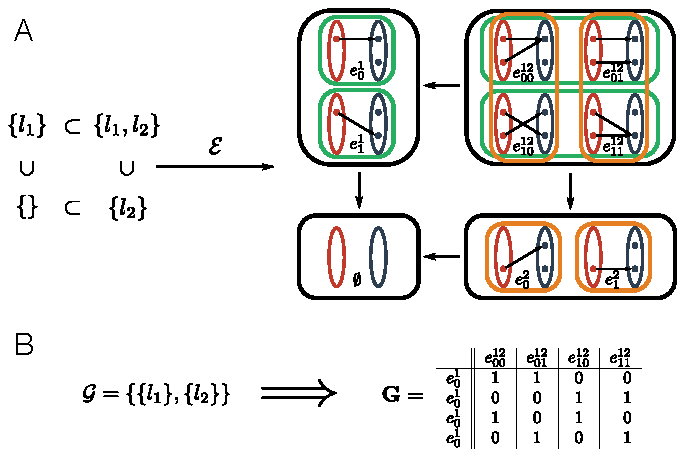
\includegraphics[width=0.8\columnwidth]{fig/efunctor.pdf}
% % \end{center}
% % $\mathcal{E}$ is thus, by definition, a presheaf functor, which is an object in the functor category $Sets^{\mathcal{P}(L)^{opp}}$.

% % Let $L$ denote a set of genes which comprise a genome like that of \ref{fig:genesallelesgrns}. Subsets of genes, $U \subseteq L$, will be used to represent which genes interact. The set of all subsets of a set $X$ is denoted $\mathcal{P}(X)$. We make $L$ into a topological space encoding these interactions by specifying the open sets $\mathcal{U}$ as a subset of $\mathcal{P}(L)$.  In the case of the simple discrete examples we will consider, we will have $\mathcal{U} = \mathcal{P}(L)$, but we want to leave open the possibility of more complicated models which might take into account the way genetic material is actually situated in physical space or the manner in which genes influence each other.

% % We will represent gene expression by constructing a sheaf over this space.  To accomplish this, we will provide a function $\expression$ which assigns to each element $U$ of $\mathcal{U}$ a probability space over the mappings from genes in $U$ to expression states \ref{tab:functors}.  This is because we eventually want to compute probabilities of various sets of gene expression states. We therefore want these collections to be closed under taking countable unions and intersections as well as under complementation.  Moreover, if $U, U' \in \mathcal{U}$ and $U \subset U'$, then, if we restrict a possible expression state of the genes in $U'$ to $U$, we obtain a possible expresion state of genes in $U$.  Hence, we will demand that $\expression$ be a functor.  Furthermore, since the physical processes that underly gene activation are local, we will require that it satisfy the sheaf condition.

% % Summarizing what we have just described more formally, we have a topological space $(L,\mathcal{U})$; associated to it is the category $(\mathcal{U}, \subseteq)$ whose objects are open sets of $L$ and whose morphisms are inclusions of open sets.  Our expression map $\expression$ is a contravriant functor from this category to the category of probability spaces.

% % \begin{table}[!ht]
% % \centering
% % \begin{tabular}{>{$}l<{$}|>{$}l<{$}|>{$}l<{$}}
% % \viable & \expression & \dist \\
% % \hline
% % \emptyset & \{\bot\} & \emptyset \\
% % \{A\} & \{\bot, a=0, a=1, (a=0) \land (a=1)\} & \{(p_0, p_1) \mid p_0 + p_1 = 1\} \\
% % \{B\} & \{\bot, b=0, b=1, (b=0) \land (b=1)\} & \{(p_0, p_1) \mid p_0 + p_1 = 1\} \\
% % \{A,B\}
% % &\begin{footnotesize} \begin{tabular}{>{$}l<{$}}
% % \{\bot, (a=0) \land (b=0), (a=0) \land (b=1),
% % (a=1) \land (b=0), (a=1) \land (b=1), \\
% % ((a=0) \land (b=0)) \lor ((a=0) \land (b=1)),
% % ((a=0) \land (b=0)) \lor ((a=1) \land (b=0)), \\
% % ((a=0) \land (b=0)) \lor ((a=1) \land (b=1)),
% % ((a=0) \land (b=1)) \lor ((a=1) \land (b=0)), \\
% % ((a=0) \land (b=1)) \lor ((a=1) \land (b=1)),
% % ((a=1) \land (b=0)) \lor ((a=1) \land (b=1)), \\
% % ((a=0) \land (b=0)) \lor ((a=0) \land (b=1)) \lor ((a=1) \land (b=0)), \\
% % ((a=0) \land (b=0)) \lor ((a=0) \land (b=1)) \lor ((a=1) \land (b=1)), \\
% % ((a=0) \land (b=0)) \lor ((a=1) \land (b=0)) \lor ((a=1) \land (b=1)), \\
% % ((a=0) \land (b=1)) \lor ((a=1) \land (b=0)) \lor ((a=1) \land (b=1)), \\
% % ((a=0) \land (b=0)) \lor ((a=0) \land (b=1)) \lor ((a=1) \land (b=0)) \lor ((a=1) \land (b=1))\}
% % \end{tabular} \end{footnotesize} & \begin{tabular}{>{$}l<{$}}
% % \{(p_{00}, p_{01}, p_{10}, p_{11}) \mid \\
% % \quad p_{00} + p_{01} + p_{10} + p_{11} = 1\} \\ \end{tabular} \\
% % \end{tabular}
% % \caption{Example of the model description. As the simplest illustration, consider a case where we have two genes, $A$ and $B$ each of which have two expression states, low and high, which we denote as $0$ and $1$.}
% % \label{tab:functors}
% % \end{table}

% \section{Stochastic genotype-phenotype maps}\label{sec:sgpm}
% There may be several sources for stochasticity in genotype-phenotype mapping including small numbers of the causal molecules and products of gene expression as well as environmental fluctuations upon which genotype-phenotype mappings are conditioned \cite{Swain2002,Paulsson2004,Thattai2004,Acar2008a,Lestas2010,Munsky2012,Chalancon2012,Neuert2013,Sanchez2013}. Regardless of the fundamental nature of stochasticity to gene expression, empirically, we observe statistical as opposed to deterministic data. Here we generalize the deterministic framework outlined above to the stochastic case.

% To accomplish this, we shall introduce probability distributions in a functorial manner.  Recall that, if $(S,\mathcal{B}(S))$ is a measurable space, then a probability measure over $(S,\mathcal{B}(S))$ is a mapping $p \colon \mathcal{B}(S) \to [0,1]$ such that $p(S) = 1$ and $p(\bigcup_{k=1}^\infty (X_k) = \sum_{k=0}^\infty p(X_k)$ for any collection $X_k$ of pairwise disjoint elements of $\mathcal{B}(S)$.  Let $\dist((S,\mathcal{B}(S)))$ denote the set of all probability distributions over $(S,\mathcal{B}(S))$.

% Furthermore, given a map between measurable spaces $(f:S \rightarrow S', f^{-1} : \mathcal{B}(S') \rightarrow \mathcal{B}(S))$ where $f$ is a projection, there is an inclusion of measurable spaces $f^{-1} : \mathcal{B}(S') \rightarrow \mathcal{B}(S))$. Given a probability distribution $p \colon \mathcal{B}(S) \to [0,1]$, the composition $p \circ f^{-1}$ is a probability distribution on $\mathcal{B}(S')$.  Let us denote this operation, which corresponds to marginalization of probabilities, as $\dist(f^{-1}) : \dist((S',\mathcal{B}(S'))) \to \dist((S,\mathcal{B}(S)))$.  With this definition, $\dist$ is a functor from the category of measurable spaces introduced in the previous section to the category $Prob$ whose objects are probability distributions and whose morphisms correspond to marginalization.

% % An \emph{algebraic structure} is determined by a set and one or more finitary operations (e.g. binary multiplication) defined on the elements of that set \cite{PachterLior2005,Artin2010}. A \emph{monoid} is a type of algebraic structure determined by a set and a binary operation such that the latter satisfies closure, associativity and identity with respect to the given set. A \emph{semiring} is an algebraic structure determined by a set with two binary operations. One of the binary operations, addition, forms a commutative monoid and has identity element 0. The second binary operation, multiplication, is a monoid with identity element 1. These binary operations interact such that multiplication distributes over addition and multiplication by the identity element of the addition monoid annihilates all elements in the semiring. For example, the real numbers under addition and multiplication constitute a semiring whose data is described as $\left( \mathbb{R},+,0,\times,1 \right)$.

% The composite $\dist \circ \expression$ is a contravariant functor from $(\mathcal{U}, \subseteq)$ to probability distributions.  However, as we shall see, this functor, unlike $\expression$, \emph{does not} satisfy the sheaf conditions and hence we only have a \emph{pre}-sheaf of probability distributions over $L$.

% For the case in which we consider the set of genes combined with the collection of all subsets of those genes we have the measurable space given by $(L,\mathcal{P}(L))$, where the probability distributions are discrete and defined over finite sets. Consider a function, $\phi$ from a set, $L$, to $\mathbb{R}$ written $\phi \colon L \rightarrow \mathbb{R}$. A distribution, $d$, on $L$ is given as a function having finite support and satisfying the constraint
% \begin{eqnarray*}
% d \colon L \rightarrow \mathbb{R},\\
% \sum_{l \in L} d(l) = 1
% \end{eqnarray*}
% We can consider the set of all distributions satisfying the above constraints and defined on the set $L$ as being given by a functor applied to $L$ as $\mathcal{D}_{\mathbb{R}} (L)$. We can again explicitly represent the way in which the functor $\mathcal{D}_{\mathbb{R}}$ acts on objects and morphisms $L$ and $f \colon L \rightarrow M$ (where $L$ and $M$ are sets viewed as sets of genes and in some special cases we may have $M=L$) as
% \begin{equation}\label{eq:distfunctor}
% \begin{split}
% \mathcal{D}_R \colon Set &\rightarrow Set,\\
% L &\mapsto \mathcal{D}_R (L),\\
% f \colon L \rightarrow M &\mapsto \mathcal{D}_R (f) \colon \mathcal{D}_R (L) \rightarrow \mathcal{D}_R (M),
% \end{split}
% \end{equation}
% where
% \begin{eqnarray*}
% \mathcal{D}_R (f) \colon \mathcal{D}_R (L) &\rightarrow& \mathcal{D}_R (M),\\
% d &\mapsto& \left[ m \mapsto \sum_{f(l)=m} d(l) \right].
% \end{eqnarray*}
% For the case in which we consider $R$ to be the semiring of non-negative real numbers $\left( \mathbb{R}_{\geq 0},+,0,\times,1 \right)$, $\mathcal{D}_R (L)$ represents the set of probability distributions over the set $L$.

% Recalling the presheaf functor, $\mathcal{E} \colon \mathcal{P}(L)^{opp} \rightarrow Set$, mapping genotypes to the set of maps from those genotypes to the set of phenotypes, we can now compose it with the distribution functor $\mathcal{D}_R$ to obtain a new presheaf functor $\mathcal{D}_R \circ \mathcal{E} \colon \mathcal{P}(L)^{opp} \rightarrow Set \rightarrow Set$ that assigns to each genotype a distribution over the set of maps from those genotypes to the set of possible phenotypes. The action of $\mathcal{D}_R \mathcal{E}$ on objects and morphisms in $\mathcal{P}(L)^{opp}$ yields
% \begin{eqnarray*}
% \mathcal{D}_R \mathcal{E} \colon \mathcal{P}(L)^{opp} &\rightarrow& Set,\\
% U &\mapsto& \mathcal{D}_R \mathcal{E}(U) \equiv d \colon P^U \rightarrow R,\\
% U \subseteq U' &\mapsto& \mathcal{D}_R \mathcal{E}(U') \rightarrow \mathcal{D}_R \mathcal{E}(U).
% \end{eqnarray*}
% where
% \begin{eqnarray*}
% \mathcal{D}_R \mathcal{E}(U') &\rightarrow& \mathcal{D}_R \mathcal{E}(U),\\
% d \colon P^{U'} \rightarrow R &\rightarrow& d|U \colon P^{U} \rightarrow R
% \end{eqnarray*}
% and
% \begin{eqnarray*}
% d \colon P^{U'} &\rightarrow& R,\\
% s' &\mapsto& d(s');\\
% d|U \colon P^{U} &\rightarrow& R,\\
% s &\mapsto& \sum_{s' \in \mathcal{E}(U'),\, s'|U=s} d(s').
% \end{eqnarray*}
% $d|U$ is a representation of what is commonly referred to as the marginal distribution of $d$ that assigns to each genotype-phenotype mapping in the smaller collection (recall $U \subseteq U'$) of such $P^{U}$ the sum of the probabilities of all genotype-phenotype maps in the larger collection $P^{U'}$ that restrict to a given map in $P^{U}$.

% If we now include the coarse-graining process from microscopic to macroscopic phenotypes we end up with the following overall relationships
% \begin{center}
% 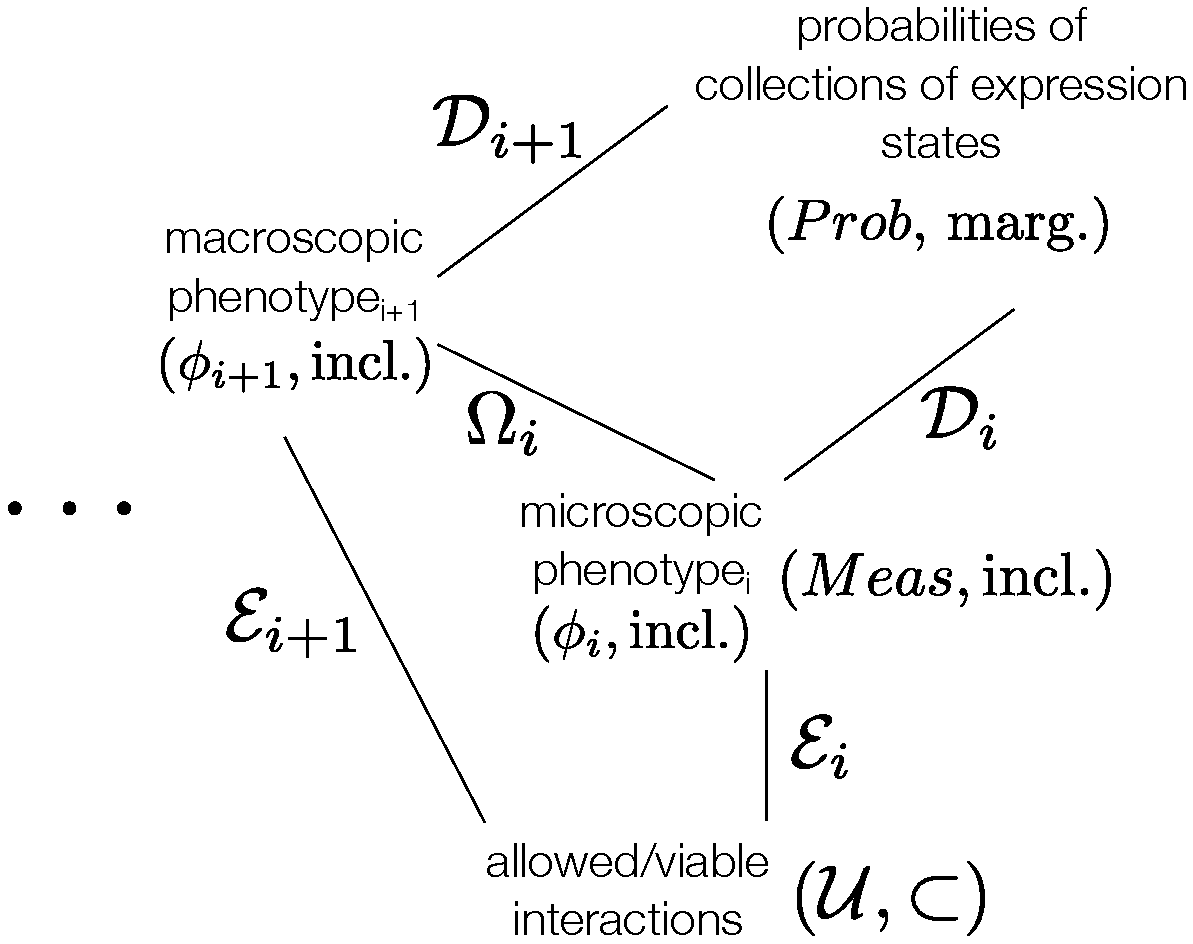
\includegraphics[width=0.4\columnwidth]{fig/abstractroadmap.pdf}
% \end{center}
% In order for the coarse-graining from lower level phenotype$_i$ to phenotype$_{i+1}$ to be a consistent one, there must be a natural transformation between the functors $\mathcal{E}_i$ and $\mathcal{E}_{i+1}$ implying that the following diagram commutes
% $$
% \xymatrix{
% \mathcal{E}_{i+1}(U_1) \ar[r]^{\mathcal{E}_{i+1}(\subseteq)} \ar[d]_{t_{U_1}} & \mathcal{E}_{i+1}(U_2) \ar[d]^{t_{U_2}} \\
% \mathcal{E}_{i}(U_1) \ar[r]^{\mathcal{E}_{i}(\subseteq)} & \mathcal{E}_{i}(U_2) }
% $$
% for any $U_2 \subseteq U_1$. For example, if our lower level phenotypes for a set of genes $U_1 = \{ l_1,l_2,l_3,l_4 \}$ are given by a set of binary sequences, then the projection of these phenotypes down to the set $U_2$ followed by mapping to the higher level phenotypes $a=\{01\}$ and $b=\{11\}$ is equivalent to first mapping to the higher-level phenotypes $A$ and $B$, indicated below, and then projecting down to $U_2$ shown by the equivalent paths from the bottom-left to the top-right in \ref{fig:phenotypehierarchy}.
% Of course, there is an equivalent diagram for the subset $\{ l_1,l_2,l_3 \}$.

\section{Gene regulatory network modules}\label{sec:covergenotypespace}
A \emph{gene regulatory network module} is represented by a subset of genes $O$ and a collection of gene regulatory network modules, whose union is the set of genes $L$, is a set of such subsets $\mathcal{G}$ (i.e. $O,O',\ldots \in \mathcal{G}$). An individual may be represented by the correlations among its genes encoded as a collection of subsets of genes. A \emph{covering} of this space of possible genes, $\mathcal{G}$, satisfies 1. $\cup_i O_i = \cup \mathcal{G} = L$ and 2. if $O,O' \in \mathcal{G}$ and $O \subseteq O'$ means that $O = O'$. This is equivalent to $\mathcal{G}$ being a reduced hypergraph, Sperner family or clutter \cite{Lauritzen1996} over $L$. The first condition means that $\mathcal{G}$ covers $L$. It is thereby just a statement that $\mathcal{G}$ represents a decomposition of the collection of all genes under consideration into subsets and this is why we refer to $\mathcal{G}$ as a collection of gene regulatory network modules. The second condition means simply that we will not consider nested subsets and so we will take for our $O \in \mathcal{G}$ the biggest $O \in \mathcal{G}$ that is not a subset of some other $O' \in \mathcal{G}$. The second condition also implies that if a given subset of genes $O'$ is compatible in a sense to be explained more precisely in what proceeds then any smaller subset of genes $O$ is also compatible. Coverings $\mathcal{G}$ of the genotype space contain the necessary information to make precise what we heuristically refer to at other points in this paper as modularity in order to cohere with standard terminology in systems biology literature while attempting to submit our own precise interpretation of the relatively colloquial concept.

\section{Compatibility of distributions on genotype-phenotype maps}\label{sec:compatibilityofgpms}
Given a covering of the genotype space $\mathcal{G}$, a compatible family for $\mathcal{G}$ with respect to the distribution presheaf $\mathcal{D}_R\mathcal{E}$ is given by a family of distributions $\{d_O \colon P^O \rightarrow R | O \in \mathcal{G}\}$ such that for all $O \in \mathcal{G}$ there exists $d_O \in \mathcal{D}_R\mathcal{E}(O)$ such that for all $O' \in \mathcal{G}$
\begin{eqnarray}\label{eq:sheafcond}
%\forall O \in \mathcal{G} \left[ \exists d_O \in \mathcal{D}_R\mathcal{E}(O) \right],\\
d_O|O \cap O' = d_{O'}|O \cap O'.
\end{eqnarray}
The condition \ref{eq:sheafcond} is referred to as the \emph{sheaf condition}. This condition means that any two distributions $d_O$ and $d_{O'}$ in the \emph{compatible family} of distributions produce the same values in the semiring $R$ on all of the genes in the intersection of $O$ with $O'$.

For example, if we have two gene regulatory network modules given by their genotypes $O = \{l_1, l_2\}$ and $O' = \{l_1, l_3\}$ then the sheaf condition specifies that for $e_{\{l_1\}} \in \mathcal{E}(\{l_1\})$, which assigns a particular phenotype to the genotype $\{l_1\}$ rather than to an entire gene regulatory network module like $O$ or $O'$, that
\begin{eqnarray}\label{eq:sheafprob}
\sum_{e \in \mathcal{E}(O),\, e|l_1=e_{\{l_1\}}} d_O(e) \,\, = \sum_{e' \in \mathcal{E}(O'),\, e'|l_1=e_{\{l_1\}}} d_{O'}(e')
\end{eqnarray}
This condition means that the probability for gene $l_1$ to be associated to the phenotype given by $e_{\{l_1\}}$ is equivalent in case we marginalize over all the other genes contained in the gene regulatory network modules of which $l_1$ is a component. For coherence with respect to the relationship between the modeling framework described here and that used in probabilistic graphical models in machine learning, the conditions \ref{eq:sheafprob} are referred to as the marginalization constraints \cite{Wainwright2007}.

\section{Global sections of distributions over genotype-phenotype maps}\label{sec:globalsectiongpms}
To say that the sheaf condition holds for a compatible family $\{d_O\}_{O \in \mathcal{G}}$ for the presheaf $\mathcal{D}_R\mathcal{E}$ implies the existence of a \emph{global section} $d \in \mathcal{D}_R\mathcal{E}(L)$ that is defined on the full set of genes. An example of a distribution that could be a global section given that it satisfies the sheaf condition is shown in \ref{tab:hidvarmod}. This global section defines a distribution on the set of genotype-phenotype maps given by $\mathcal{E}(L) = P^L$, specifying phenotypes associated to all genes at once instead of on subsets of $L$ associated to either $U \subseteq L$ or, what is essentially equivalent, $O \in \mathcal{G}$. Crucially, the distribution $d$ must also restrict for the subset of genes associated to any gene regulatory network module, which in some cases may represent all of the genes in an organism, $O$ in a covering of the genotype space $\mathcal{G}$ meaning that
\begin{eqnarray}
\forall O \in \mathcal{G} \left[ d|O = d_O \right].
\end{eqnarray}
In terms of distributions, the existence of a global section $d$ for a covering of the genotype space $\mathcal{G}$ corresponds to the existence of a distribution defined on all genes that marginalizes to yield the distributions on subsets of genes that may be observed empirically.

The presheaf $\mathcal{E}$ alone was already a sheaf because given a cover $\{U_i\}_{i \in I}$ of $U$ there is a family of sections $\{e_i \in \mathcal{E}(U_i)\}_{i \in I}$ that is compatible in the sense that
\begin{eqnarray}
\forall i,j \in I \left[ e_i|U_i \cap U_j = e_j|U_i \cap U_j \right].
\end{eqnarray}
In this case there is a unique global section $e \in \mathcal{E}(U)$ such that $\forall i \in I \left[ e|U_i = e_i \right]$. The fact that the sheaf condition holds for $\mathcal{E}$ is true because we are considering functions defined on a space with a trivial discrete topology allowing us to combine any partial functions that agree on overlapping subsets by taking the union of the data defining such functions.

Extending this example on an arbitrary subset $U \subseteq L$ to the whole set of genes $L$ we have a unique global section $e \in \mathcal{E}(L) = P^L$. $e$ can be used to deterministically assign phenotypes to the set of genes $L$ under consideration.

